\section{Probability Using Tree Diagrams and Combinations}\label{section_probability_tree_and_combinations}

In this section, you will learn to:
\begin{enumerate}
    \item Use probability tree diagrams to calculate probabilities.
    \item Use combinations to calculate probabilities.
\end{enumerate}

In this section, we will apply previously learned counting techniques in calculating probabilities and use tree diagrams to help us gain a better understanding of what is involved.

\subsection{Using Tree Diagrams to Calculate Probabilities}

We already used tree diagrams to list events in a sample space. Tree diagrams can be helpful in organizing information in probability problems; they help provide a structure for understanding probability. In this section, we expand our previous use of tree diagrams to situations in which the events in the sample space are not all equally likely.

We assign the appropriate probabilities to the events shown on the branches of the tree. By multiplying probabilities along a path through the tree, we can find probabilities for "and" events, which are intersections of events.

We begin with an example.

\begin{example}\label{example_drawing_marbles_with_replacement}
    Suppose a jar contains 3 red and 4 white marbles. If two marbles are drawn with replacement, what is the probability that both marbles are red?
\end{example}
\begin{solution}
    Let \( E \) be the event that the first marble drawn is red, and let \( F \) be the event that the second marble drawn is red.

    We need to find \( P(E \cap F) \). By the statement, "two marbles are drawn with replacement," we mean that the first marble is replaced before the second marble is drawn.

    There are 7 choices for the first draw. Since the first marble is replaced before the second is drawn, there are again seven choices for the second draw. Using the multiplication axiom, we conclude that the sample space \( S \) consists of 49 ordered pairs. Of the 49 ordered pairs, there are \( 3 \cdot 3 = 9 \) ordered pairs that show red on the first draw and, also, red on the second draw. Therefore,
    \[ P(E \cap F) = \frac{9}{49} \]

    Further note that in this particular case
    \[ P(E \cap F) = \frac{9}{49} = \frac{3}{7} \cdot \frac{3}{7} \]

    giving us the result that in this example: \( P(E \cap F) = P(E) \cdot P(F) \)
\end{solution}

\begin{example}
    If we use the same 3 red and 4 white marbles from Example \ref{example_drawing_marbles_with_replacement}, but the two marbles are drawn \textbf{without} replacement, what is the probability that both marbles are red?
\end{example}

\begin{solution}
    By the statement, "two marbles are drawn without replacement," we mean that the first marble is not replaced before the second marble is drawn.

    There are, again, 7 choices for the first draw but since the first marble is not replaced before the second is drawn, there are only six choices for the second draw. Using the multiplication axiom, we conclude that the sample space \( S \) consists of 42 ordered pairs. Of the 42 ordered pairs, there are \( 3 \cdot 2 = 6 \) ordered pairs that show red on the first draw and red on the second draw. Therefore,
    \[ P(E \cap F) = \frac{6}{42} \]

    Note that we can break this calculation down as
    \[ P(E \cap F) = \frac{6}{42} = \frac{3}{7} \cdot \frac{2}{6} \]

    Here \( \frac{3}{7} \) represents \( P(E) \), and \( \frac{2}{6} \) represents the probability of drawing a red on the second draw, given that the first draw resulted in a red.
\end{solution}

We write the latter as \( P(\text{red on the second} \mid \text{red on first}) \) or \( P(F \mid E) \). The ``$|$'' represents the word ``given'' or ``if''. This is an important result, called the Multiplication Rule, which will appear again in later sections.

\begin{summarybox}{Multiplication Rule}
    \[ P(E \cap F) = P(E) \cdot P(F \mid E) \]
\end{summarybox}


We now demonstrate the above results with a tree diagram.

\begin{example}
    Suppose a jar contains 3 red and 4 white marbles. If two marbles are drawn without replacement, find the following probabilities using a tree diagram:
    \begin{enumerate}
        \item The probability that both marbles are red.
        \item The probability that the first marble is red and the second white.
        \item The probability that one marble is red and the other white.
    \end{enumerate}
\end{example}

\begin{solution}
    Let \( R \) be the event that the marble drawn is red, and let \( W \) be the event that the marble drawn is white.
    We draw the following tree diagram:

    \begin{center}
        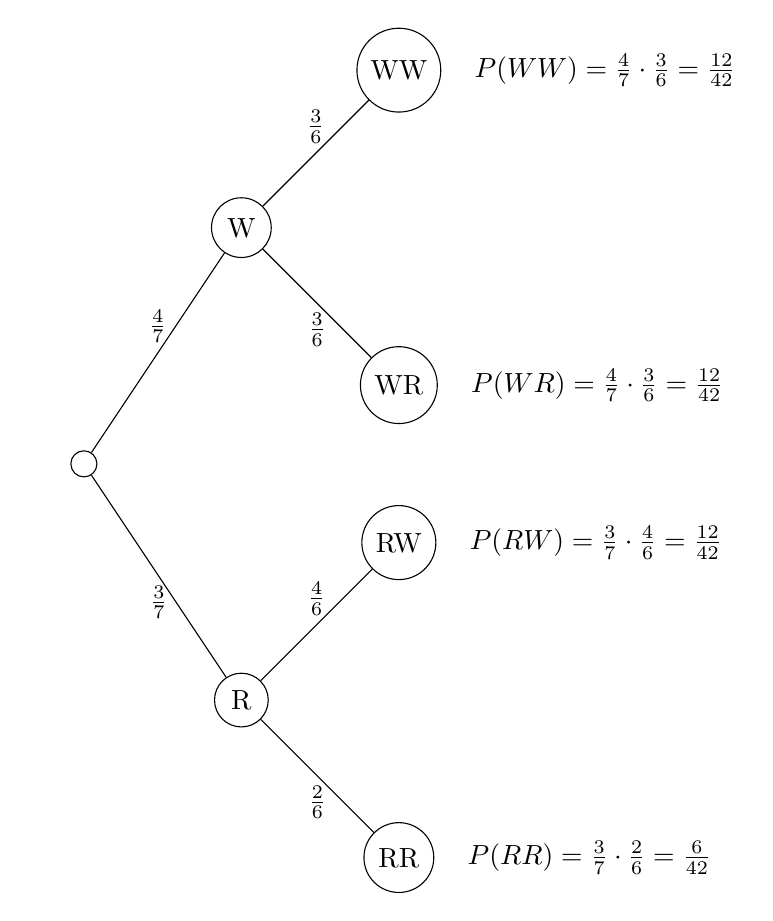
\begin{tikzpicture}[grow=right, label distance=3mm]
            \tikzstyle{level 1}=[level distance=2cm, sibling distance=6cm]
            \tikzstyle{level 2}=[level distance=2cm, sibling distance=4cm]
            \node[circle, draw, label=left:{}] {}
            child {
            node[circle, draw, label=above:{}] {R}
            child {
            node[circle, draw, label=right:{$P(RR) = \frac{3}{7}\cdot\frac{2}{6} = \frac{6}{42}$}] {RR}
            edge from parent
            node[below] {$\frac{2}{6}$
                }
            }
            child {
            node[circle, draw, label=right:{$P(RW) = \frac{3}{7}\cdot\frac{4}{6} = \frac{12}{42}$}] {RW}
            edge from parent
            node[above] {$\frac{4}{6}$}
            }
            edge from parent
            node[below] {$\frac{3}{7}$}
            }
            child {
            node[circle, draw, label=below:{}] {W}
            child {
            node[circle, draw, label=right:{$P(WR) = \frac{4}{7}\cdot\frac{3}{6} = \frac{12}{42}$}] {WR}
            edge from parent
            node[below] {$\frac{3}{6}$
                }
            }
            child {
            node[circle, draw, label=right:{$P(WW) = \frac{4}{7}\cdot\frac{3}{6} = \frac{12}{42}$}] {WW}
            edge from parent
            node[above] {$\frac{3}{6}$
                }
            }
            edge from parent
            node[above] {$\frac{4}{7}$}
            };
        \end{tikzpicture}
    \end{center}

    \begin{enumerate}
        \item The probability that both marbles are red is \[ P(RR) = \frac{6}{42} \]

        \item The probability that the first marble is red and the second is white is

              \[ P(RW) = \frac{12}{42} \]

        \item For the probability that one marble is red and the other is white, we observe that this can be satisfied if the first is red and the second is white, or if the first is white and the second is red. The ``or'' tells us we'll be using the Addition Rule from Section \ref{section_mutually_exclusive_events_and_addition_rule}.

              Furthermore events RW and WR are mutually exclusive events, so we use the form of the Addition Rule that applies to mutually exclusive events.

              Therefore

              \[
                  P(\text{one marble is red and the other marble is white})
              \]
              \[
                  = P(RW \text{ or } WR) = P(RW) + P(WR)
              \]
              \[
                  = \frac{12}{42} + \frac{12}{42}
              \]
              \[
                  = \frac{24}{42}.
              \]

    \end{enumerate}
\end{solution}

\subsection{Using Combinations to Find Probabilities}
Although the tree diagrams give us better insight into a problem, they are not practical for problems where more than two or three things are chosen.  In such cases, we use the concept of combinations that we learned in the last chapter.   This method is best suited for problems where the order in which the objects are chosen is not important, and the objects are chosen without replacement.


\begin{example}
    Suppose a jar contains 3 red, 2 white, and 3 blue marbles. If three marbles are drawn without replacement, find the following probabilities.
    \begin{enumerate}
        \item \( P(\text{Two red and one white}) \)
        \item \( P(\text{One of each color}) \)
        \item \( P(\text{None blue}) \)
        \item \( P(\text{At least one blue}) \)
    \end{enumerate}
\end{example}

\begin{solution}
    Let us suppose the marbles are labeled as \[ R_1, R_2, R_3, W_1, W_2, B_1, B_2, B_3. \]
    \begin{enumerate}
        \item Since we are choosing 3 marbles from a total of 8, there are \( 8C3 \) possible combinations. Of these \( 8C3 \) combinations, there are \( 3C3 \cdot 2C1 \) combinations consisting of 2 red and one white. Thus,
              \[ P(\text{Two red and one white}) = \frac{3C2 \cdot 2C1}{8C3} = \frac{6}{56} = \frac{3}{28}. \]

        \item For one of each color, there are \( 8C3 \) possible combinations. Of these $56$ combinations, there are $3C1 \cdot 2C1 \cdot 3C1 = 18$ combinations consisting of one red, one white, and one blue.  we have
              \[ P(\text{One of each color}) = \frac{3C1 \cdot 2C1 \cdot 3C1}{8C3} = \frac{18}{56} = \frac{9}{28}\].

        \item For none blue, there are 5 non-blue marbles, so \[ P(\text{None blue}) = \frac{5C3}{8C3} = \frac{10}{56}= \frac{5}{28}\].

        \item By ``at least one blue marble'', we mean the following: one blue marble and two non-blue marbles, or two blue marbles and one non-blue marble, or all three blue marbles. So we have to find the sum of the probabilities of all three cases.

              \[
                  P(\text{At least one blue}) = P(1 \text{ blue, } 2 \text{ non-blue}) + P(2 \text{ blue, } 1 \text{ non-blue}) + P(3 \text{ blue})
              \]
              \[
                  P(\text{At least one blue}) = \frac{3C1 \cdot 5C2}{8C3} + \frac{3C2 \cdot 5C1}{8C3} + \frac{3C3}{8C3}
              \]
              \[
                  P(\text{At least one blue}) = \frac{30}{56} + \frac{15}{56} + \frac{1}{56} = \frac{46}{56} = \frac{23}{28}.
              \]

              Alternatively, for at least one blue, we can use the complement rule where \( P(E) = 1 - P(\overline{E}) \) because the opposite of ``at least one blue'' is ``none blue''. Given \( P(\text{None blue}) \) from our previous work, we have \[ P(\text{At least one blue}) = 1 - P(\text{None blue}) = 1- \frac{5}{28} = \frac{23}{28}.\]
    \end{enumerate}
\end{solution}

\begin{example}
    Five cards are drawn from a deck. Find the probability of obtaining two pairs, that is, two cards of one value, two of another value, and one other card.
\end{example}

\begin{solution}
    Let us first do an easier problem—the probability of obtaining a pair of kings and queens. Since there are four kings, and four queens in the deck, the probability of obtaining two kings, two queens and one other card is
    \[ P(\text{A pair of kings and queens}) = \frac{4C2 \cdot 4C2 \cdot 44C1}{52C5} \]

    To find the probability of obtaining two pairs, we have to consider all possible pairs. Since there are altogether 13 values, that is, aces, deuces, and so on, there are 13C2 different combinations of pairs.
    \[ P(\text{Two pairs}) = 13C2 \cdot \frac{4C2 \cdot 4C2 \cdot 44C1}{52C5} = .04754 \]
\end{solution}

\begin{example}
    A cell phone store receives a shipment of 15 cell phones that contains 8 iPhones and 7 Android phones. Suppose that 6 cell phones are randomly selected from this shipment. Find the probability that a randomly selected set of 6 cell phones consists of 2 iPhones and 4 Android phones.
\end{example}

\begin{solution}
    There are \( 8C2 \) ways of selecting 2 out of the 8 iPhones and \( 7C4 \) ways of selecting 4 out of the 7 Android phones. But altogether there are \( 15C6 \) ways of selecting 6 out of 15 cell phones. Therefore, we have
    \[ P(2 \text{iPhones and 4 Android}) = \frac{8C2 \cdot 7C4}{15C6} = \frac{(28)(35)}{5005} = \frac{980}{5005} = 0.1958 \]
\end{solution}

\begin{example}
    One afternoon, a bagel store still has 53 bagels remaining: 20 plain, 15 poppyseed, and 18 sesame seed bagels. Suppose that the store owner packages up a bag of 9 bagels to bring home for tomorrow’s breakfast, and selects the bagels randomly. Find the probability that the bag contains 4 plain, 3 poppyseed, and 2 sesame seed.
\end{example}

\begin{solution}
    There are \( 20C4 \) ways of selecting 4 out of the 20 plain bagels, \( 15C3 \) ways of selecting 3 out of the 15 poppyseed bagels, and \( 18C2 \) ways of selecting 2 out of the 18 sesame seed bagels. But altogether there are \( 53C9 \) ways of selecting 9 out of the 53 bagels. Therefore, we have
    \[ P(4 \text{ plain, 3 poppyseed, and 2 sesame seed}) \]
    \[= \frac{20C4 \cdot 15C3 \cdot 18C2}{53C9} = \frac{(4845)(45)(153)}{443161350} = 0.761 \]
\end{solution}

We end the section by solving a famous problem called the Birthday Problem.

\begin{example}
    If there are 25 people in a room, what is the probability that at least two people have the same birthday?
\end{example}

\begin{solution}
    Let event \( E \) represent that at least two people have the same birthday.

    We first find the probability that no two people have the same birthday.

    We analyze as follows. Suppose there are 365 days to every year. According to the multiplication axiom, there are \( 365^{25} \) possible birthdays for 25 people. Therefore, the sample space has \( 365^{25} \) elements. We are interested in the probability that no two people have the same birthday. There are 365 possible choices for the first person and since the second person must have a different birthday, there are 364 choices for the second, 363 for the third, and so on. Therefore,
    \[ P(\text{No two have the same birthday}) = \frac{365 \cdot 364 \cdot \ldots \cdot 341}{365^{25}} = \frac{365P25}{365^{25}} \]

    Since \( P(\text{at least two people have the same birthday}) = 1 - P(\text{No two have the same birthday}) \),
    \[ P(\text{at least two people have the same birthday}) = 1 - \frac{365P25}{365^{25}} \approx .5687 \]
\end{solution}

This means that a teacher can supplement their meager income by betting classes of 25 students \$100 that at least two of them share a birthday. We call the amount a teacher can expect to win on average an ``expected value''. In this case, the expected value is \$13.74. This is discussed further in Section \ref{section_expected_value}.